\documentclass[11pt]{article}

\usepackage[norsk]{babel}
\usepackage[utf8]{inputenc}
\usepackage{amsmath, amssymb, amsthm}
\usepackage{graphicx, float}
\usepackage{pstricks-add}


\author{Kjetil Kjeka}
\title{TTK4130 - Exercise 6}
\date{\today}


%Slik at matriser kan defineres med linjer
\makeatletter
\renewcommand*\env@matrix[1][*\c@MaxMatrixCols c]{%
  \hskip -\arraycolsep
  \let\@ifnextchar\new@ifnextchar
  \array{#1}}
\makeatother

\newcommand{\abs}[1]{|#1|} 


\begin{document}
\maketitle
\section*{Problem 1}
For the system
\begin{eqnarray*}
\dot{u} &=& u (v-3) \\
\dot{v} &=& c (2-u)
\end{eqnarray*}
And the ``energy like'' function
\[V = u - 2 \ln{u} + v - 3 \ln{v} \]
\subsection*{a}
\[\dot{V} = u(v-3) - \frac{2}{u} u(v-3) + v(2-u) - \frac{3}{v} v(2-u) \]
\[\dot{V} = uv - 3u - 2v + 6 + 2v -vu - 6 + 3u = 0 \]
We don't got any theorems for what happends when function which is not positive definite derivate is not negative definite.

\subsection*{b}
Simulation of the Lotka-Voltera system for 20 timeunits is given in Figure \ref{fig:LotkaVoltera}
\begin{figure}[h!]
\centering
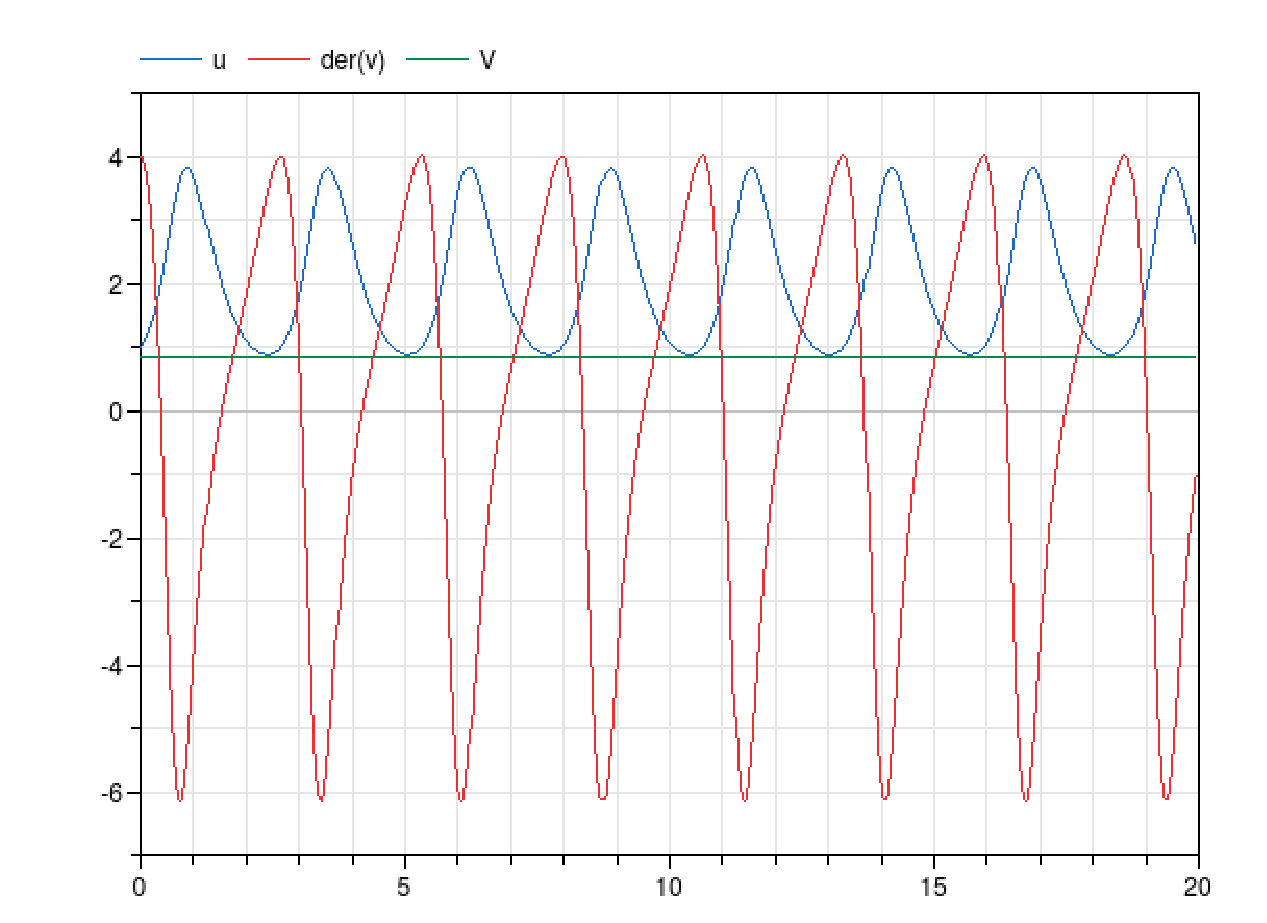
\includegraphics[width=.8\textwidth]{LotkaVoltera.eps}
\caption{Lotka-Voltera simulated for 20 time units}
\label{fig:LotkaVoltera}
\end{figure}

\subsection*{c}
The first order derivatives are:
\begin{eqnarray*}
\frac{df}{du} &=& \begin{bmatrix} v-3 \\ -v \end{bmatrix} \\
\frac{df}{dv} &=& \begin{bmatrix} u \\ 2-u \end{bmatrix} 
\end{eqnarray*}
Thus the linearization is:
\begin{eqnarray*}
\dot{u^*} &=&  2v \\
\dot{v^*} &=& -3u
\end{eqnarray*}
Which makes the eigenvalues
\[\lambda_{1,2} = \pm \sqrt{6} i \]
Which makes sense from Figure \ref{fig:LotkaVoltera} since the natural frequency $\omega$ is given by $\lambda = j\omega$ meaning $T = \frac{2 \pi}{\omega} = 2.6$

\subsection*{d}
The simulated models using the timestep $h = 0.05$ is given in Figure \ref{fig:LV_eeu} \ref{fig:LV_ieu} and \ref{fig:LV_imp}

\begin{figure}[h!]
\centering
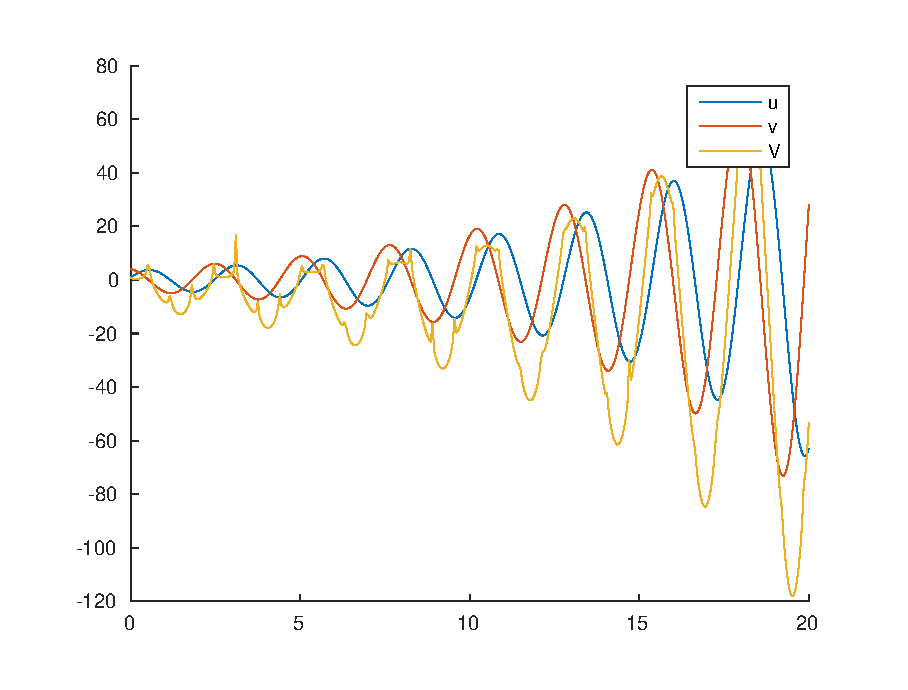
\includegraphics[width=.8\textwidth]{LV_eeu.eps}
\caption{Lotka-Voltera lineartization simulated for 20 time units with eulers method}
\label{fig:LV_eeu}
\end{figure}

\begin{figure}[h!]
\centering
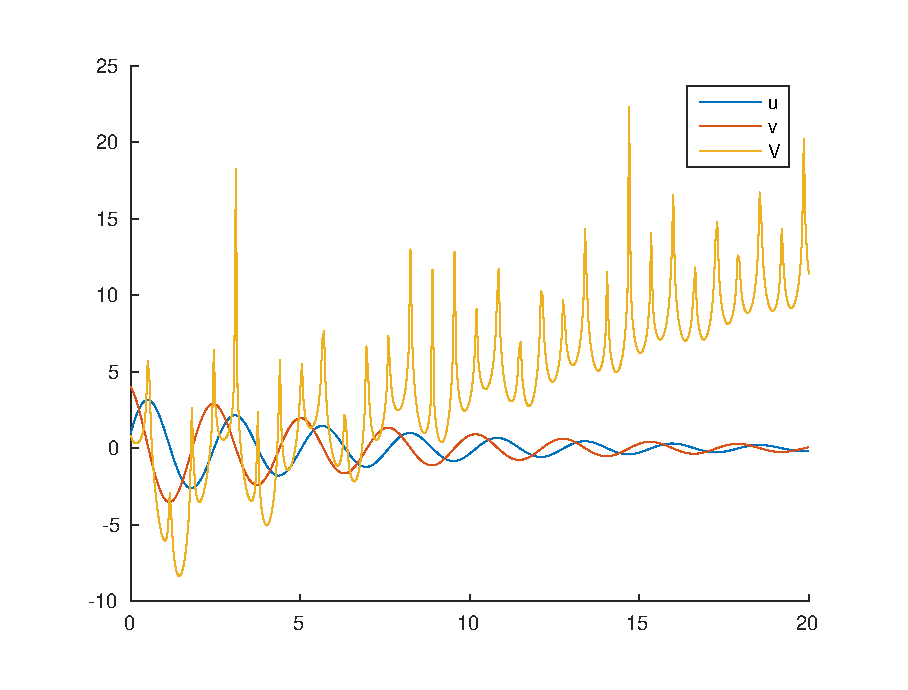
\includegraphics[width=.8\textwidth]{LV_ieu.eps}
\caption{Lotka-Voltera lineartization simulated for 20 time units with implicit eulers method}
\label{fig:LV_ieu}
\end{figure}

\begin{figure}[h!]
\centering
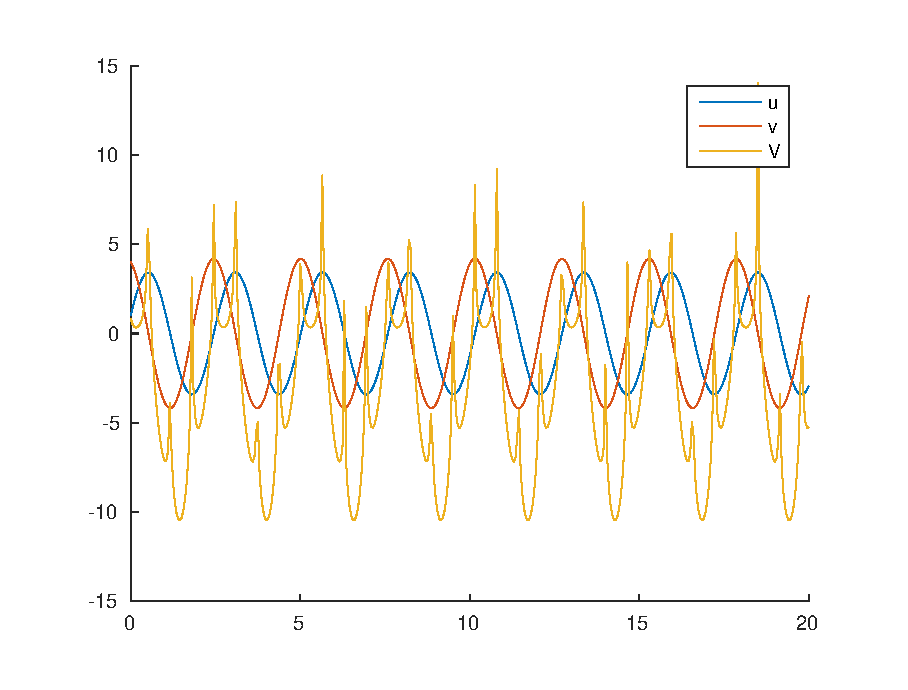
\includegraphics[width=.8\textwidth]{LV_imp.eps}
\caption{Lotka-Voltera lineartization simulated for 20 time units with implicit midpoint method}
\label{fig:LV_imp}
\end{figure}

\section*{Problem 2}
\subsection*{a}
Assuming that it is reffered to the second order method $A = \begin{bmatrix}
0 & 0 \\
\frac{3}{4} & \frac{1}{4} 
\end{bmatrix}
$, $b=\begin{bmatrix} \frac{1}{2} \\ \frac{1}{2}
\end{bmatrix}
$, $c= \begin{bmatrix} 0 \\ 1 
\end{bmatrix}
$. The stability function is thus:
\[R = \frac{\det{\mathbf{I} - \lambda h (\mathbf{A} - \mathbf{1} \mathbf{b}^T)}}{\det{(\mathbf{I} - \lambda h \mathbf{A})}} \]
For it to be A-stable then $\abs{R} < 1, \forall \lambda$ where $Re{\lambda} \leq 0$
\begin{eqnarray*}
R(h\lambda) &=& \frac{\det{\mathbf{I} - \lambda h (\mathbf{A} - \mathbf{1} \mathbf{b}^T)}}{\det{(\mathbf{I} - \lambda h \mathbf{A})}} \\
&=& \frac{\det{
\begin{bmatrix}
1 & 0 \\
0 & 1
\end{bmatrix}
- \lambda h (
\begin{bmatrix}
0 & 0 \\
\frac{1}{2} & \frac{1}{2}
\end{bmatrix}
-
\begin{bmatrix}
\frac{1}{2} & \frac{1}{2} \\
\frac{1}{2} & \frac{1}{2}
\end{bmatrix}
) } }{ \det{
\begin{bmatrix}
1 & 0 \\
0 & 1
\end{bmatrix}
- \lambda h
\begin{bmatrix}
0 & 0 \\
\frac{1}{2} & \frac{1}{2}
\end{bmatrix}
}} \\
&=& \frac{ \det{
\begin{bmatrix}
1 + \frac{1}{2}\lambda h &  \frac{1}{2} \lambda h \\
0 & 1
\end{bmatrix}
}}{\det{
\begin{bmatrix}
1 & 0 \\
\frac{1}{2} \lambda h & 1 + \frac{1}{2}\lambda h
\end{bmatrix}
}} \\
&=& \frac{1 + \frac{1}{2} \lambda h}{1 - \frac{1}{2} \lambda h} \\
&=& \frac{1 + Re(\frac{1}{2} \lambda h) + Im(\frac{1}{2} \lambda h)j}{1 - Re(\frac{1}{2} \lambda h) - Im(\frac{1}{2} \lambda h)}    
\end{eqnarray*}
Using that $Re(\lambda) \leq 0$, its sufficient to show that
\[\abs{R} = \sqrt{\frac{(1 + Re(\frac{1}{2}\lambda h))^2 + (Im(\frac{1}{2}\lambda h))^2}{(1 - Re(\frac{1}{2}\lambda h))^2 + (Im(\frac{1}{2}\lambda h))^2}} \leq 1 \]
Which is the same as showing
\[ (1 + Re(\frac{1}{2}\lambda h))^2 + (Im(\frac{1}{2}\lambda h))^2 \leq (1 - Re(\frac{1}{2}\lambda h))^2 + (Im(\frac{1}{2}\lambda h))^2 \]
Which again is the same as showing
\[ (1 + Re(\lambda))^2 \leq (1 - Re(\lambda))^2 \]
Which is true since $Re(\lambda) \leq 0$

\subsection*{b}
Since it's already shown that the method is A stable it's L stable iff $\abs{R(\lambda h)} \rightarrow 0$ when $\lambda \rightarrow \inf$
\[\lim_{\lambda \rightarrow \inf} \abs{R} = \lim_{\lambda \rightarrow \inf} \abs{\frac{1 + \frac{1}{2} \lambda h}{1 - \frac{1}{2} \lambda h}} = \lim_{\lambda \rightarrow \inf} \abs{\frac{\frac{1}{2} \lambda h}{-\frac{1}{2} \lambda h}} \]
Using L'hopital
\[\lim_{\lambda \rightarrow \inf} \abs{R} = \abs{\frac{\frac{1}{2}h}{-\frac{1}{2}h}} = 1 \]
Since $\lim_{\lambda \rightarrow \inf} \abs{R} \not = 0$ the method is not L stable


\section*{Problem 3}
\subsection*{a}
This is an implicit method because $A$ is not a lower triangular matrix.


\end{document}